\chapter{Basic definitions and results}
\setcounter{page}{1}
\pagenumbering{arabic}

\section{Preliminaries from the theory of abelian fields}
\begin{definition}
An \textit{abelian field} is a finite Galois extension of $\Q$ with an abelian Galois group. 
\end{definition}

\begin{theorem}[Kronecker-Weber]
Every abelian field is a subfield of some cyclotomic field $\Q(\zeta_n)$, where $n\in \Nbb$ and $\z_n$ is an $n$-th primitive root of unity.
\end{theorem}
\begin{proof}
See \citep{washington1997}, page 321.
%\citep{washington1982}, page 319.
\end{proof}

\begin{definition}
Let $k$ be an abelian field. The least number $n\in\mathbb{N}$ such that $k\subseteq \Q(\zeta_n)$ is called the conductor of $k$ and denoted by $\cond(k)$.
\end{definition}

\begin{rem}\label{ramif}
Using ramification theory, it's not hard to see that for any abelian field $k$, $\Q(\z_\cond(k))$ is ramified exactly at the same primes as $k$. In other words, a prime divides $\cond(k)$ iff it ramifies in $k$.
\end{rem}

\begin{definition}\label{genusdef}
The \textit{genus field in the narrow sense} of an abelian field is its maximal field extension which is abelian over $\Q$ and unramified at all finite primes.
\end{definition}

Usually, we will use Definition \ref{genusdef} only indirectly, thanks to the following lemma:
%Because Definition \ref{genusdef} is not constructive, it will prove useful to have an alternate characterization. % of the genus field in the narrow sense.
\begin{lemma}\label{genus}
Let $k$ be an abelian field, $K$ be its genus field in the narrow sense, $P$ be the set of ramified primes of $k$ and for any $p\in P$, let $e_p$ be ramification index of $p$ in $k$ and let $T_p$ be the inertia subgroup of $\Gal(K/\Q)$ corresponding to $p$. Moreover for any $p\in P$, let $K_p$ be the maximal subfield of $K$ ramified only at $p$.
%be an abelian field of degree $[K_p:\Q]=e_p$ ramified only at $p$. 
Then the following statements hold (the products denote the composita of fields):
%Assume that all the inertia subgroups of $\Gal(K/\Q)$ are cyclic and for any $p\in P$, let $K_p$ be the unique abelian field of degree $[K_p:\Q]=e_p$ ramified only at $p$. Then the following are equivalent (the products denote the composita of fields):
\begin{enumerate}[label={\upshape(\roman*)}]
%\item $K$ is the genus field in the narrow sense of $k$ (using Definition \ref{genusdef}),
\item $K=\prod_{p\in P} K_p$,
\item $K=k\prod_{p\in P\setminus \{q\}} K_p$ for any $q\in P$,
\item $\Gal(K/\Q)\cong \prod_{p\in P} T_p$ and for any $p\in P$, $$T_p=\Gal\left(K/\prod_{q\in P\setminus\{p\}}K_p\right)\cong \Gal\left(k/k\cap\prod_{q\in P\setminus\{p\}}K_p\right)\cong \Gal(K_p/\Q),$$
\item For any $p\in P$, we have $[K_p:\Q]=e_p$.
%\item For any $p\in P$, $K_p$ is the maximal subfield of $K$ ramified only at $p$.
\end{enumerate}
% $K$ is the genus field in the narrow sense of an abelian field $k$ and $P$ is the set of ramified primes of $k$, we have $\Gal(K/\Q)\cong \prod_{p\in P} T_p$, where $T_p$ is the inertia subgroup of $\Gal(K/\Q)$ corresponding to $p$.
\end{lemma}
\pagebreak
\begin{proof}
The lemma %whole equivalence \enquote{(i) $\Leftrightarrow$ (ii) $\Leftrightarrow$ (iii)} 
is well known and follows from the isomorphism of the lattice of all abelian fields and the lattice of all finite subgroups of the group of all Dirichlet characters. More specifically, Theorem 3.5 from \citep{washington1997}, page 24 %or 23 in 1st ed
is used in the proof. %We will briefly outline only the proof of (ii) and omit the rest.
\end{proof}

\begin{rem}
\iffalse
\begin{DESCRIPTION}%[labelindent=0cm]
\item[\enquote{(ii)+(iii) $\Leftrightarrow$ (iv)}:] This follows by elementary Galois theory, since $K_p\cap K_q=\Q$ for any $p,q\in P$.
\item[\enquote{(ii) $\Leftrightarrow$ (v)}:] This is clear from the definition of ramification.
\item[\enquote{(i) $\Rightarrow$ (iii)}:] 
\end{DESCRIPTION}
\fi
We will at least briefly outline the proof of (ii) in Lemma \ref{genus}.
Let $q\in P$ be fixed.
The extension $K/\prod_{p\in P\setminus\{q\}}K_p$ is totally ramified at the prime ideals above $q$, so the same must be true for the extension $K/k\prod_{p\in P\setminus\{q\}}K_p$. But since the extension $K/k$ is unramified by the definition of $K$, so is $K\!/\!k\prod_{p\in P\setminus\{q\}}K_p$. Therefore $[K:k\prod_{p\in P\setminus\{q\}}K_p]\!=\!1$.
\begin{center}
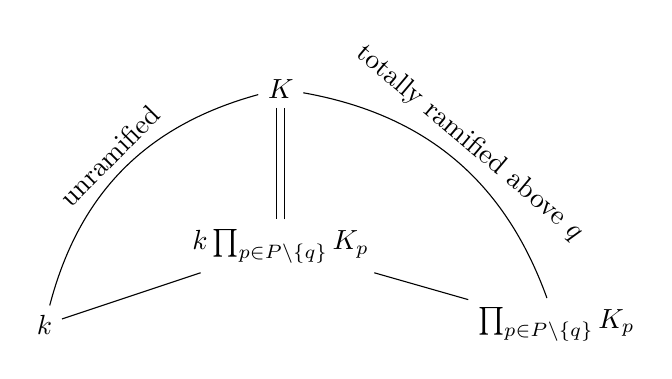
\begin{tikzpicture}
  \node (a) at (0,4)  {$K$};
  \node (b) at (0,2)  {$k\prod_{p\in P\setminus\{q\}}K_p$};
  \node (c) at (-3,1)  {$k$};
  \node (d) at (3.5,1)  {$\prod_{p\in P\setminus\{q\}}K_p$};
  \draw[transform canvas={xshift=-1.5pt}] (a) -- (b);
  \draw[transform canvas={xshift=1.5pt}] (b) -- (a);
  \draw   (b) --  (c)
   (b) -- (d);
  \draw[bend left](c) to node [above , sloped]{\text{unramified}}(a);
  \draw[bend right](d) to node [above , sloped]{\text{totally ramified above $q$}}(a);
\end{tikzpicture}
\end{center}
\end{rem}

\begin{rem}
Note that for any odd $p\in P$, the field $K_p$ in the statement of Lemma \ref{genus} is determined uniquely by the condition (iv) alone (together with the fact that it must be abelian), because by Remark \ref{ramif},%the ramification requirement,
 it must be a subfield of the cyclotomic field $\Q(\zeta_{p^f})$ for some $f\in\Nbb$, whose absolute Galois group is isomorphic to $(\Z/p^f\Z)^{\times}$, which is cyclic, since $p$ is odd. Thus if only odd primes ramify in $k$, the equalities (i) or (ii) in Lemma \ref{genus} can be used to construct $K$ from $k$. In general though, this argument doesn't help us determine the field $K_2$ without prior knowledge of $K$ (there could be up to three possibilities), and the \enquote{correct} choice of $K_2$ is given by the theory of Dirichlet characters. However, even in this case we can still construct $K$ only from the data provided by $k$ thanks to the equality (ii).
 
 %iff $p\geq 3$ or $f\leq 2$, and cyclic groups have at exactly one quotient group of any possible order. %The assumption of the cyclicity of all inertia groups in the statement of the lemma is thus not required for $p\geq 3$ or $f\leq 2$, and can be also be removed for the other cases (but then there are three possible choices for $K_2$, so we must slightly change the statement).
\end{rem}

\iffalse
\begin{lemma}\label{comp}
We have $kK_iK_jK_l=K$ and $K_1K_2K_3K_4=K$.
\end{lemma}
\begin{proof}
The extension $K/K_iK_jK_l$ is totally ramified at the prime ideals above $p_h$, so the same must be true for the extension $K/kK_iK_jK_l$. But since the extension $K/k$ is unramified (by the definition of $K$), so is $K/kK_iK_jK_l$. Therefore $[K:kK_iK_jK_l]=1$. The second claim follows from the facts %$\Gal(K_i/\Q)\cong$
$T_i=\Gal(K/K_jK_lK_h)$ and $G=T_1\times T_2\times T_3\times T_4$.
\end{proof}
\begin{center}
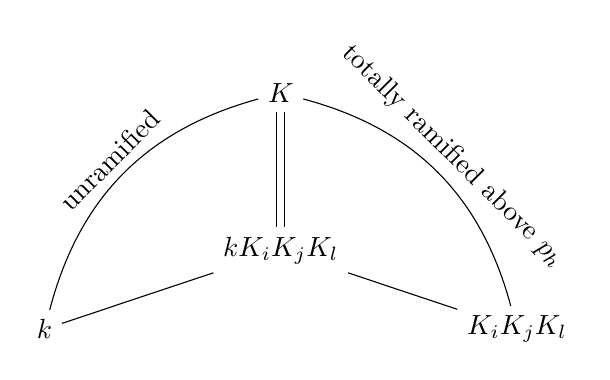
\begin{tikzpicture}
  \node (a) at (0,4)  {$K$};
  \node (b) at (0,2)  {$kK_iK_jK_l$};
  \node (c) at (-3,1)  {$k$};
  \node (d) at (3,1)  {$K_iK_jK_l$};
  \draw[transform canvas={xshift=-1.5pt}] (a) -- (b);
  \draw[transform canvas={xshift=1.5pt}] (b) -- (a);
  \draw   (b) --  (c)
   (b) -- (d);
  \draw[bend left](c) to node [above , sloped]{\text{unramified}}(a);
  \draw[bend right](d) to node [above , sloped]{\text{totally ramified above $p_h$}}(a);
\end{tikzpicture}
\end{center}
\fi

\begin{definition}
An element $\alpha$ of a real abelian field $K$ is called \textit{totally positive} if for any embedding $\sigma: K\to \R$, we have $\sigma(\alpha)>0$.
\end{definition}

\section{The groups of circular numbers and circular units}
\begin{definition}
Let $G$ be any group. The (integral) \textit{group ring} $\Z[G]$ is the free $\Z$-module with basis $G$, which is made into a ring, extending linearly the group law on $G$.
\end{definition}

For the remainder of this chapter, let $k\neq \Q$ be a real abelian field, $K$ be its the genus field in the narrow sense, $P$ be the set of ramified primes of $k$ (note that the condition $k\neq \Q$ implies that $P\neq \emptyset$) and $K_p$ be the maximal subfield of $K$ ramified only at $p\in P$. Since $\Gal(K/\Q)$ has a natural action on $K$ (given by evaluating an automorphism on an element), this makes $K$ into a $\Z[\Gal(K/\Q)]$-module. 

The following definition is equivalent to Lettl's modification of Sinnott's definition:
\begin{definition}
The group $D(k)$ of circular numbers of $k$ is given as
$$D:=\big\langle \{-1\} \cup \{\eta_I \big\vert \emptyset \subsetneq I \subseteq P \}\big\rangle_{\Z[\Gal(K/\Q)]},$$
where $\langle \dots \rangle_{\Z[\Gal(K/\Q)]}$ means \enquote{generated as a $\Z[\Gal(K/\Q)]$-submodule of $K$} and $$\eta_I=\text{N}_{\Qbb(\zeta_{\text{cond} \left(\prod_{i\in I}K_i\right)})/\left(\prod_{i\in I}K_i\right)\cap k}\left(1-\zeta_{\text{cond} \left(\prod_{i\in I}K_i\right)}\right),$$ where $\text{N}$ denotes the norm operator and the product of fields denotes their compositum. The subgroup of totally positive elements of $D(k)$ will be denoted by $D^+(k)$.
\end{definition}

\begin{definition}
The group $C(k)$ of circular numbers of $k$ is $E(k)\cap D(k)$, where $E(k)$ is the group of units of the ring of algebraic integers of $k$. The subgroup of totally positive elements of $C(k)$ will be denoted by $C^+(k)$.
\end{definition}

\begin{rem}
All the generators $\eta_I$ of $D(k)$ are norms of nonzero elements from an imaginary abelian field to a real subfield. Hence for any $I$, we can write 
$$\eta_I=(1-\z_{\cond(\prod_{i\in I}K_i)})^{\sum_{i=1}^r(\sigma_i+\overline{\sigma_i})}$$
for some $r\in\Nbb$, where $\overline{\sigma_i}$ is the automorphism which is complex conjugate to $\sigma_i$. It follows that $\sigma(\eta_I)>0$ for any embedding $\sigma:k\to \R$, so that $\eta_I$ so totally positive. On the other hand, $-1$ is not totally positive and its product with any totally positive element is also not totally positive. This shows that $$D^+(k)=\big\langle  \eta_I \big\vert \emptyset \subsetneq I \subseteq P\big\rangle_{\Z[\Gal(K/\Q)]},$$
which is canonically isomorphic to the to torsion-free part of $D(k)$. Since $\Z$ is a principal ideal domain and $D(k)$ is finitely generated, this implies that $D^+(k)$ and consequently also $C^+(k)$ are free $\Z$-modules.
\end{rem}

In \citep{Lettl1990}, it is proven that the previous definition of $C(k)$ gives the same group as Sinnott's original definition in \citep{SinnottAb}. One of the reasons that $C(k)$ is important is the following result, due to Sinnott:
\begin{theorem}\label{finind}
The index $[E(k):C(k)]$ is finite.
\end{theorem}
\begin{proof}
See \citep{SinnottAb}, Theorem 4.1.
\end{proof}

\begin{lemma}\leavevmode \label{units}
Let  $\emptyset \subsetneq I \subseteq P$.
\begin{enumerate} [label={\upshape(\roman*)}]
\item For $|I|>1$, we have $\eta_I\in E(k)$.
\item For $|I|=1$, we have $\eta_I\not\in E(k)$, but $\eta_I^{1-\sigma}\in E(k)$ for any $\sigma\in \Gal(K/\Q)$. % in the inertia subgroup of $\Gal(K/\Q)$ corresponding to $p$.
\end{enumerate}
\end{lemma}
\begin{proof}
Let $n=\cond(\prod_{i\in I}K_i)$. Since $\eta_I$ is a norm of the algebraic integer $1-\z_n$, it is also an algebraic integer, so it suffices to compute its absolute norm to prove (i).
%Also for any $\sigma\in \Gal(K/\Q)$, the commutitavity of $\Gal(K/\Q)$ implies that $\eta_I^{1-\sigma}$ is a norm of $(1-\z_n)^{1-\sigma}$
%Since all $\eta_I$ are algebraic integers, it suffices to compute their absolute norm. 
We have 
\begin{align*}
\N_{\prod_{i\in I}K_i\cap k/\Q}(\eta_I)=\N_{\Qbb(\z_n)/\Q}(1-\z_n)=
\begin{cases}
p & \quad \text{ if } n \text{ is a power of a prime } p,\\
1 & \quad \text{ otherwise } \\
\end{cases}
\end{align*}
using the computation in \citep{Sedlacek2015thesis}, page 29. Since $\Q(\z_n)$ is ramified at the same primes as $\prod_{i\in I}K_i$ by Remark \ref{ramif}, it follows that $\N_{\prod_{i\in I}K_i\cap k/\Q}(\eta_I)=1$ iff $|I|>1$.

As for (ii), note that for any $\sigma\in \Gal(K/\Q)$, the commutitavity of $\Gal(K/\Q)$ implies that $\eta_I^{1-\sigma}$ is a norm of $(1-\z_n)^{1-\sigma}$. But $(1-\z_n)^{1-\sigma}=\frac{1-\z_n}{1-\z_n^a}$ for some $a\in\Z$, $\gcd(a,n)=1$, and by Lemma 3.9 in \citep{Sedlacek2015thesis}, this is a unit. Since the norm of a unit is again a unit, we are done.
%for any $\sigma\in \Gal(K/\Q)$, we have $\N_{\prod_{i\in I}K_i\cap k/\Q}(\eta_I)=\N_{\prod_{i\in I}K_i\cap k/\Q}(\sigma(\eta_I))$, hence $\N_{\prod_{i\in I}K_i\cap k/\Q}(\eta_I^{1-\sigma})=1$, which proves the rest of the assertion.
%This follows from \citep{SinnottAb}, Lemma 4.1. %nebo bakalářka?
\end{proof}

\begin{cor}
We have $$C(k)=\big\langle \{ -1\}\cup \{\eta_I \big\vert I \subseteq P,  |I|\geq 2\} \cup \{\eta_I^{1-\sigma} \big\vert |I|=1, \sigma\in \Gal(K/\Q))\}\big\rangle_{\Z[\Gal(K/\Q]}$$
and
$$C^+(k)=\big\langle \{ \eta_I \big\vert I \subseteq P,  |I|\geq 2\} \cup \{\eta_I^{1-\sigma} \big\vert |I|=1, \sigma\in \Gal(K/\Q))\}\big\rangle_{\Z[\Gal(K/\Q]}.$$
\end{cor}

\begin{prop}\label{Drank}
The $\Z$-rank of $D^+(k)$ is $[k:\Q]+|P|-1$ and the $\Z$-rank of $C^+(k)$ is $[k:\Q]-1$.
\end{prop}
\begin{proof}
By Dirichlet's unit theorem, the $\Z$-rank of $E(k)$ is $[k:\Q]-1$, since all the embeddings of $k$ are real. Since the index $[E(k):C(k)]$ is finite by Theorem \ref{finind},  the $\Z$-rank of $C(k)$ must be $[k:\Q]-1$ as well. Since $C^+(k)$ is isomorphic to the torsion-free part of $C(k)$, its $\Z$-rank must also be $[k:\Q]-1$
%Because $C(k)$ is finitely generated, its torsion subgroup is finite, hence the $\Z$-rank of $C^+(k)$, which is isomorphic to the non-torsion part of $C(k)$ by Lemma \ref{torsion}, must also be $[k:\Q]-1$.

Now consider the quotient module $D^+(k)/C^+(k)$. By Lemma \ref{units}, it is generated as a $\Z$-module by the images of $\eta_I$ for $|I|=1$, hence it has exactly $|P|$ generators. Since the absolute norm of $\eta_{\{p\}}$ is a power of $p$%odkaz na bakalářku?
, the elements $\eta_I$ with $|I|=1$ are multiplicatively independent (any nontrivial relation between them would give us a nontrivial multiplicative relation between powers of different primes, which is not possible). Moreover, since the absolute norm of all elements in $C^+(k)$ is $1$, the images of $\eta_I$ remain multiplicatively independent in $D^+(k)/C^+(k)$. Thefore this quotient module has $\Z$-rank $|P|$, which implies that the $\Z$-rank of $D^+$ is $[k:\Q]+|P|-1$ by the first part.
\end{proof}

\begin{lemma}\label{NoFrob}
If $L' \subset L$ are abelian fields, then for any $\epsilon\in C(L)$ (resp. $C^+(L)$, resp. $D(L)$, resp. $D^+(L)$) we have $\N_{L/L'}(\epsilon)\in C(L')$ (resp. $C^+(L')$, resp. $D(L')$, resp. $D^+(L')$).
\end{lemma}
\begin{proof}
This is well known and can be proved easily using the original Sinnott's definition of $C(L)$.
\end{proof}

%\subsection{Odstavec}

